%\textual
\chapter{A Arquitetura Proposta}

Este capítulo é dividido em três seções, a primeira realiza uma contextualização da proposta, a segunda o mapeamento das entidades e relacionamentos do modelo PROV-DM para o modelo de um banco de dados de grafo e a terceira especifica a arquitetura de armazenamento de proveniência.

\section{Contextualização da Proposta}

Como apresentado no capítulo anterior, existem na literatura trabalhos usando os modelos de proveniência OPM e PROV-DM, armazenamento dos dados de proveniência em bancos de dados de grafos e proveniência de dados para processos executados em um ambiente de computação em nuvem, porém não tratam de um modelo de dados para proveniência de \textit{workflow} de Bioinformática usando bancos de dados de grafos para armazenar os dados do modelo PROV-DM com execução em um ambiente de computação em nuvem. Neste contexto, os principais aspectos que levaram a definição desta arquitetura são:

\begin{itemize}
\item Como apresentado em \cite{renato}, o modelo PROV-DM pode ser aplicado em \textit{workflow} de Bioinformática onde através de um grafo é possível facilmente representar a proveniência em um experimento da Bioinformática;
\item Como o PROV-DM é um modelo baseado em grafo, onde toda proveniência pode ser representada através de nós e arestas, este trabalho propõe como contribuição o armazenamento dos dados de proveniência em um banco de dados de grafo;
\item A execução do \textit{workflow} em um ambiente de computação em nuvem é uma realidade em vários experimentos na Bioinformática, devido as característica de elasticidade, redução de custo na aquisição e composição de toda infraestrutura e prover uma abstração e facilidade de acesso aos usuários.
\end{itemize}

\section{Modelo de dados de proveniência no NoSQL baseado em bancos de dados de grafo}

Banco de dados de grafos permitem o armazenamento de entidades e relacionamentos entre essas entidades, que também são conhecidas como nodos, os quais possuem propriedades. Os relacionamentos são conhecidos como arestas que também podem ter propriedades. As arestas têm significância direcional; nodos são organizados por relacionamentos, os quais permitem encontrar padrões entre eles.

Sendo assim os dois tipos básicos do modelo PROV-DM, atividade e entidade serão representados como nodos no banco de dados de grafo, e serão diferenciados pela propriedade Tipo. Já as relações serão representadas pelas arestas no banco de dados de grafo, sendo diferenciadas também por uma propriedade Tipo. Logo, teremos o seguinte modelo:

\begin{figure}[h!]
\centering
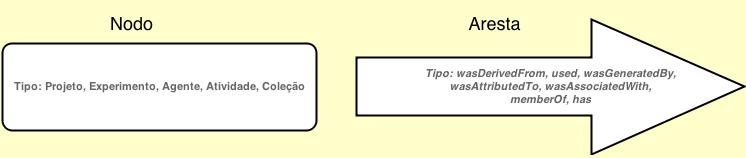
\includegraphics[width=350pt]{images/NodoEAresta.jpg}
\caption{Mapeamento dos tipos e relações para o modelo de dados baseado em grafo.}
\label{fig:nodoaresta}
\end{figure}

Na Figura \ref{fig:modeloneoj} tem-se o mapeamento mais detalhado dos tipos de entidades do modelo PROV-DM e dados de proveniência para o banco de dados de grafo. Pode-se observar o acréscimo de duas entidades que não pertencem ao modelo PROV-DM: Projeto e Experimento, são necessárias porque existe a necessidade de agrupar vários experimentos em um mesmo projeto para facilitar o compartilhamento do grafo de proveniência gerado. Essa mesma idéia é aplicada entre as entidades Experimento e Atividades.

\begin{figure}[h!]
\centering
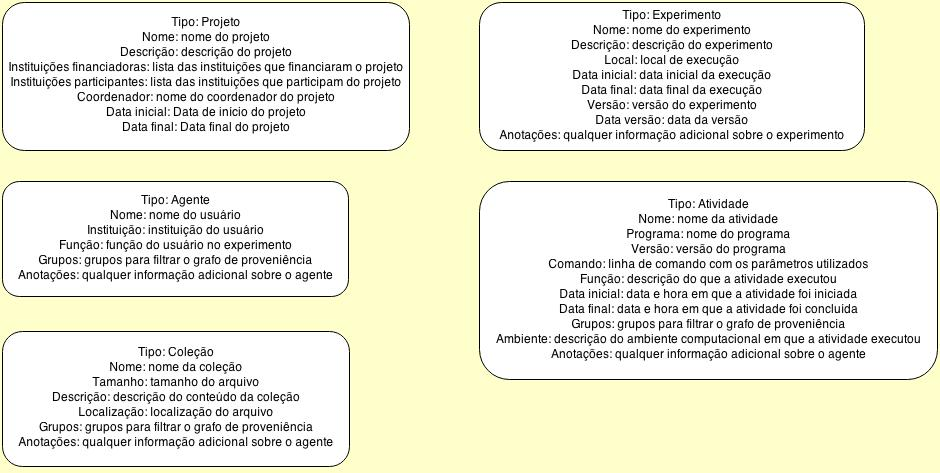
\includegraphics[width=450pt]{images/ModeloNeo4J.jpg}
\caption{Mapeamento dos tipos e relações para um modelo de grafos.}
\label{fig:modeloneoj}
\end{figure}

\section{Arquitetura proposta}

O objetivo desta seção é definir uma arquitetura para a coleta de proveniência de dados em projetos de bioinformática de forma automática para o ambiente de computação em nuvem usando o modelo PROV-DM.

Na Figura \ref{fig:arquitetura} pode-se ver os principais componentes da arquitetura: 

\begin{itemize}
\item Uma interface web simples e amigável para o usuário, permitindo-o criar projetos, experimentos e atividades. Os dados informados pelo usuário serão enviados para a nuvem para serem processados;
\item Módulo de execução: responsável por executar os comandos ou programas recebidos do usuário;
\item Módulo de captura de dados de proveniência: responsável por receber os dados informados pelo usuário e interpretá-los e realizar a captura da proveniência de forma automática;
\item Módulo de armazenamento: será responsável pela comunicação com o banco de dados de grafo e prover uma interface de acesso;
\item Banco de dados de grafo: responsável pelo armazenamento dos dados na forma de grafo.
\end{itemize}

\begin{figure}[h!]
\centering
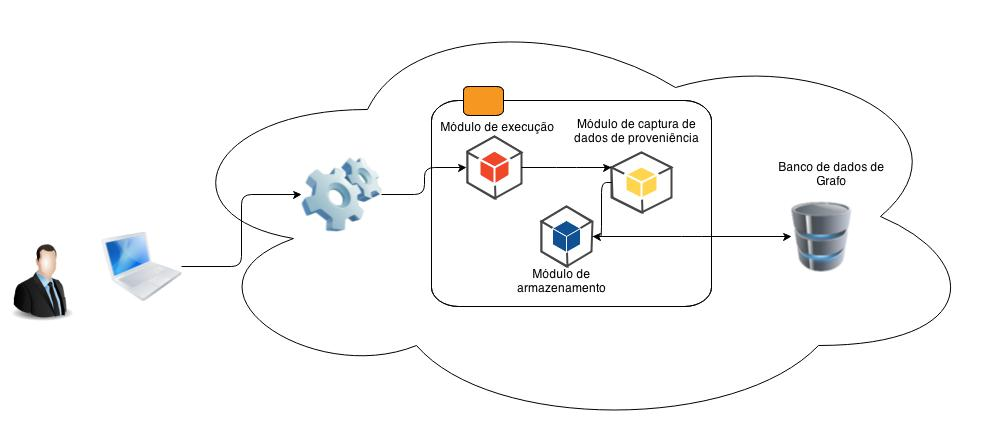
\includegraphics[width=450pt]{images/ArquiteturaPropostaII.jpg}
\caption{Arquitetura Proposta.}
\label{fig:arquitetura}
\end{figure}

%\section{Neo4J}
% De acordo com \cite{neo4j}, os bancos de dados de grafos operam em nodos conectados, a maioria das soluções, geralmente, não suporta a distribuição de nodos em servidores diferentes. Porém, há algumas soluções, que suportam a distribuição de nodos em um \textit{cluster} de servidores, como o \textit{Neo4J}. Ao executá-lo em um \textit{cluster}, uma gravação no mestre acaba sendo sincronizada com os escravos, enquanto que os escravos estão sempre disponíveis para a leitura. Gravações nos escravos são permitidas e imediatamente sincronizadas com o mestre; outros escravos, porém, não serão sincronizados imediatamente, eles terão de esperar que os dados se propaguem a partir do mestre.

% O Neo4J é compatível com as propriedades ACID (acrônimo para Atomicidade, Consistência, Isolamento e Durabilidade). Antes de alterar quaisquer nodos ou adicionar algum relacionamento a nodos já existentes \cite{neo4j}.

% Segundo \cite{fowler}, o Neo4J obtém alta disponibilidade ao permitir escravos replicados a partir da versão 1.8. Esses escravos também podem lidar com gravações: quando algo é gravado neles, eles sincronizam a gravação com o mestre atual e essa gravação é confirmada, primeiro no mestre e depois no escravo. Outros escravos receberão a atualização eventualmente.

% Pode-se encontrar \cite{fowler}, que o Neo4J possuia a linguagem de consulta \textit{Gremlin}, que é uma linguagem específica de domínio para percorrer grafos, o \textit{Cypher}, que é uma outra linguagem de consulta para pesquisar no grafo. O \textit{Cypher} precisa de um nodo \textit{START} para iniciar a consulta, utiliza a palavra-chave \textit{MATCH} para buscar padrões em relacionamentos; a palavra-chave \textit{WHERE} filtra as propriedades em um nodo ou relacionamento e a palavra-chave \textit{RETURN} especifica o que é  retornado pela consulta. Além destas linguagens de consulta, o \textit{Neo4J} permite que você consulte propriedades dos nodos do grafo, ou percorra os relacionamentos dos nodos utilizando \textit{bindings} da linguagem.

% Ainda segundo \cite{fowler} há três maneiras de fazer os bancos de dados em grafos crescerem em escala. A primeira é adicionar mais memória ao servidor, de modo que o conjunto de nodos e relacionamentos sendo trabalhados esteja inteiramente na memória. A segunda forma é melhorar o desempenho na leitura do banco de dados adicionando aos dados mais escravos com acesso apenas a leitura, com todas as gravações sendo enviadas para o mestre. E por último, quando o tamanho do conjunto de dados torna impraticável a replicação, pode-se fragmentar os dados a partir do lado do aplicativo utilizando o conhecimento específico do domínio.
